\chapter{Diagramma delle classi}

\section{Package SimulazioneF1}
\vspace{2cm}

\begin{figure}[h!]
    \centering
    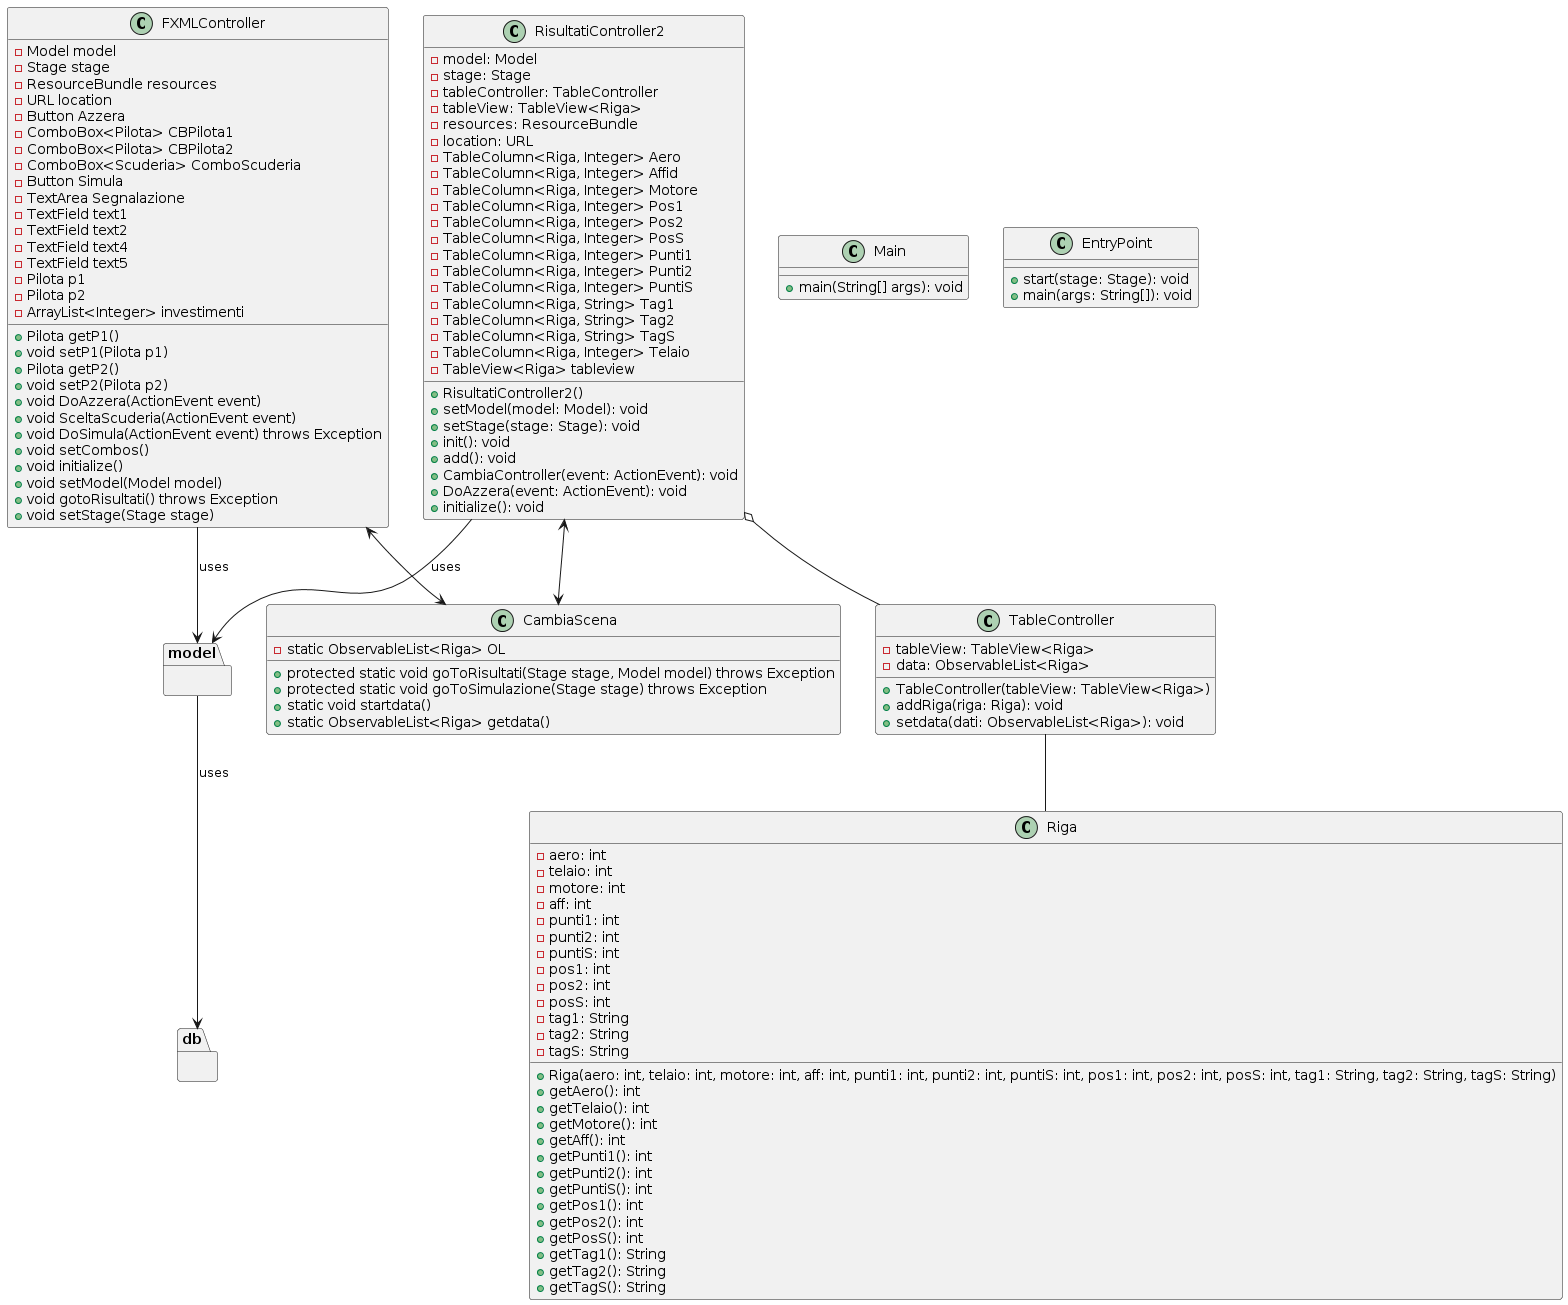
\includegraphics[width=\linewidth]{Figures/uml1.png}
    \caption{Diagramma UML del package SimulazioneF1}
    \label{fig:diagramma_simulazionef1}
\end{figure}
\newpage
\section{Package SimulazioneF1.model}
\vspace{1cm}
\begin{figure}[h!]
    \centering
    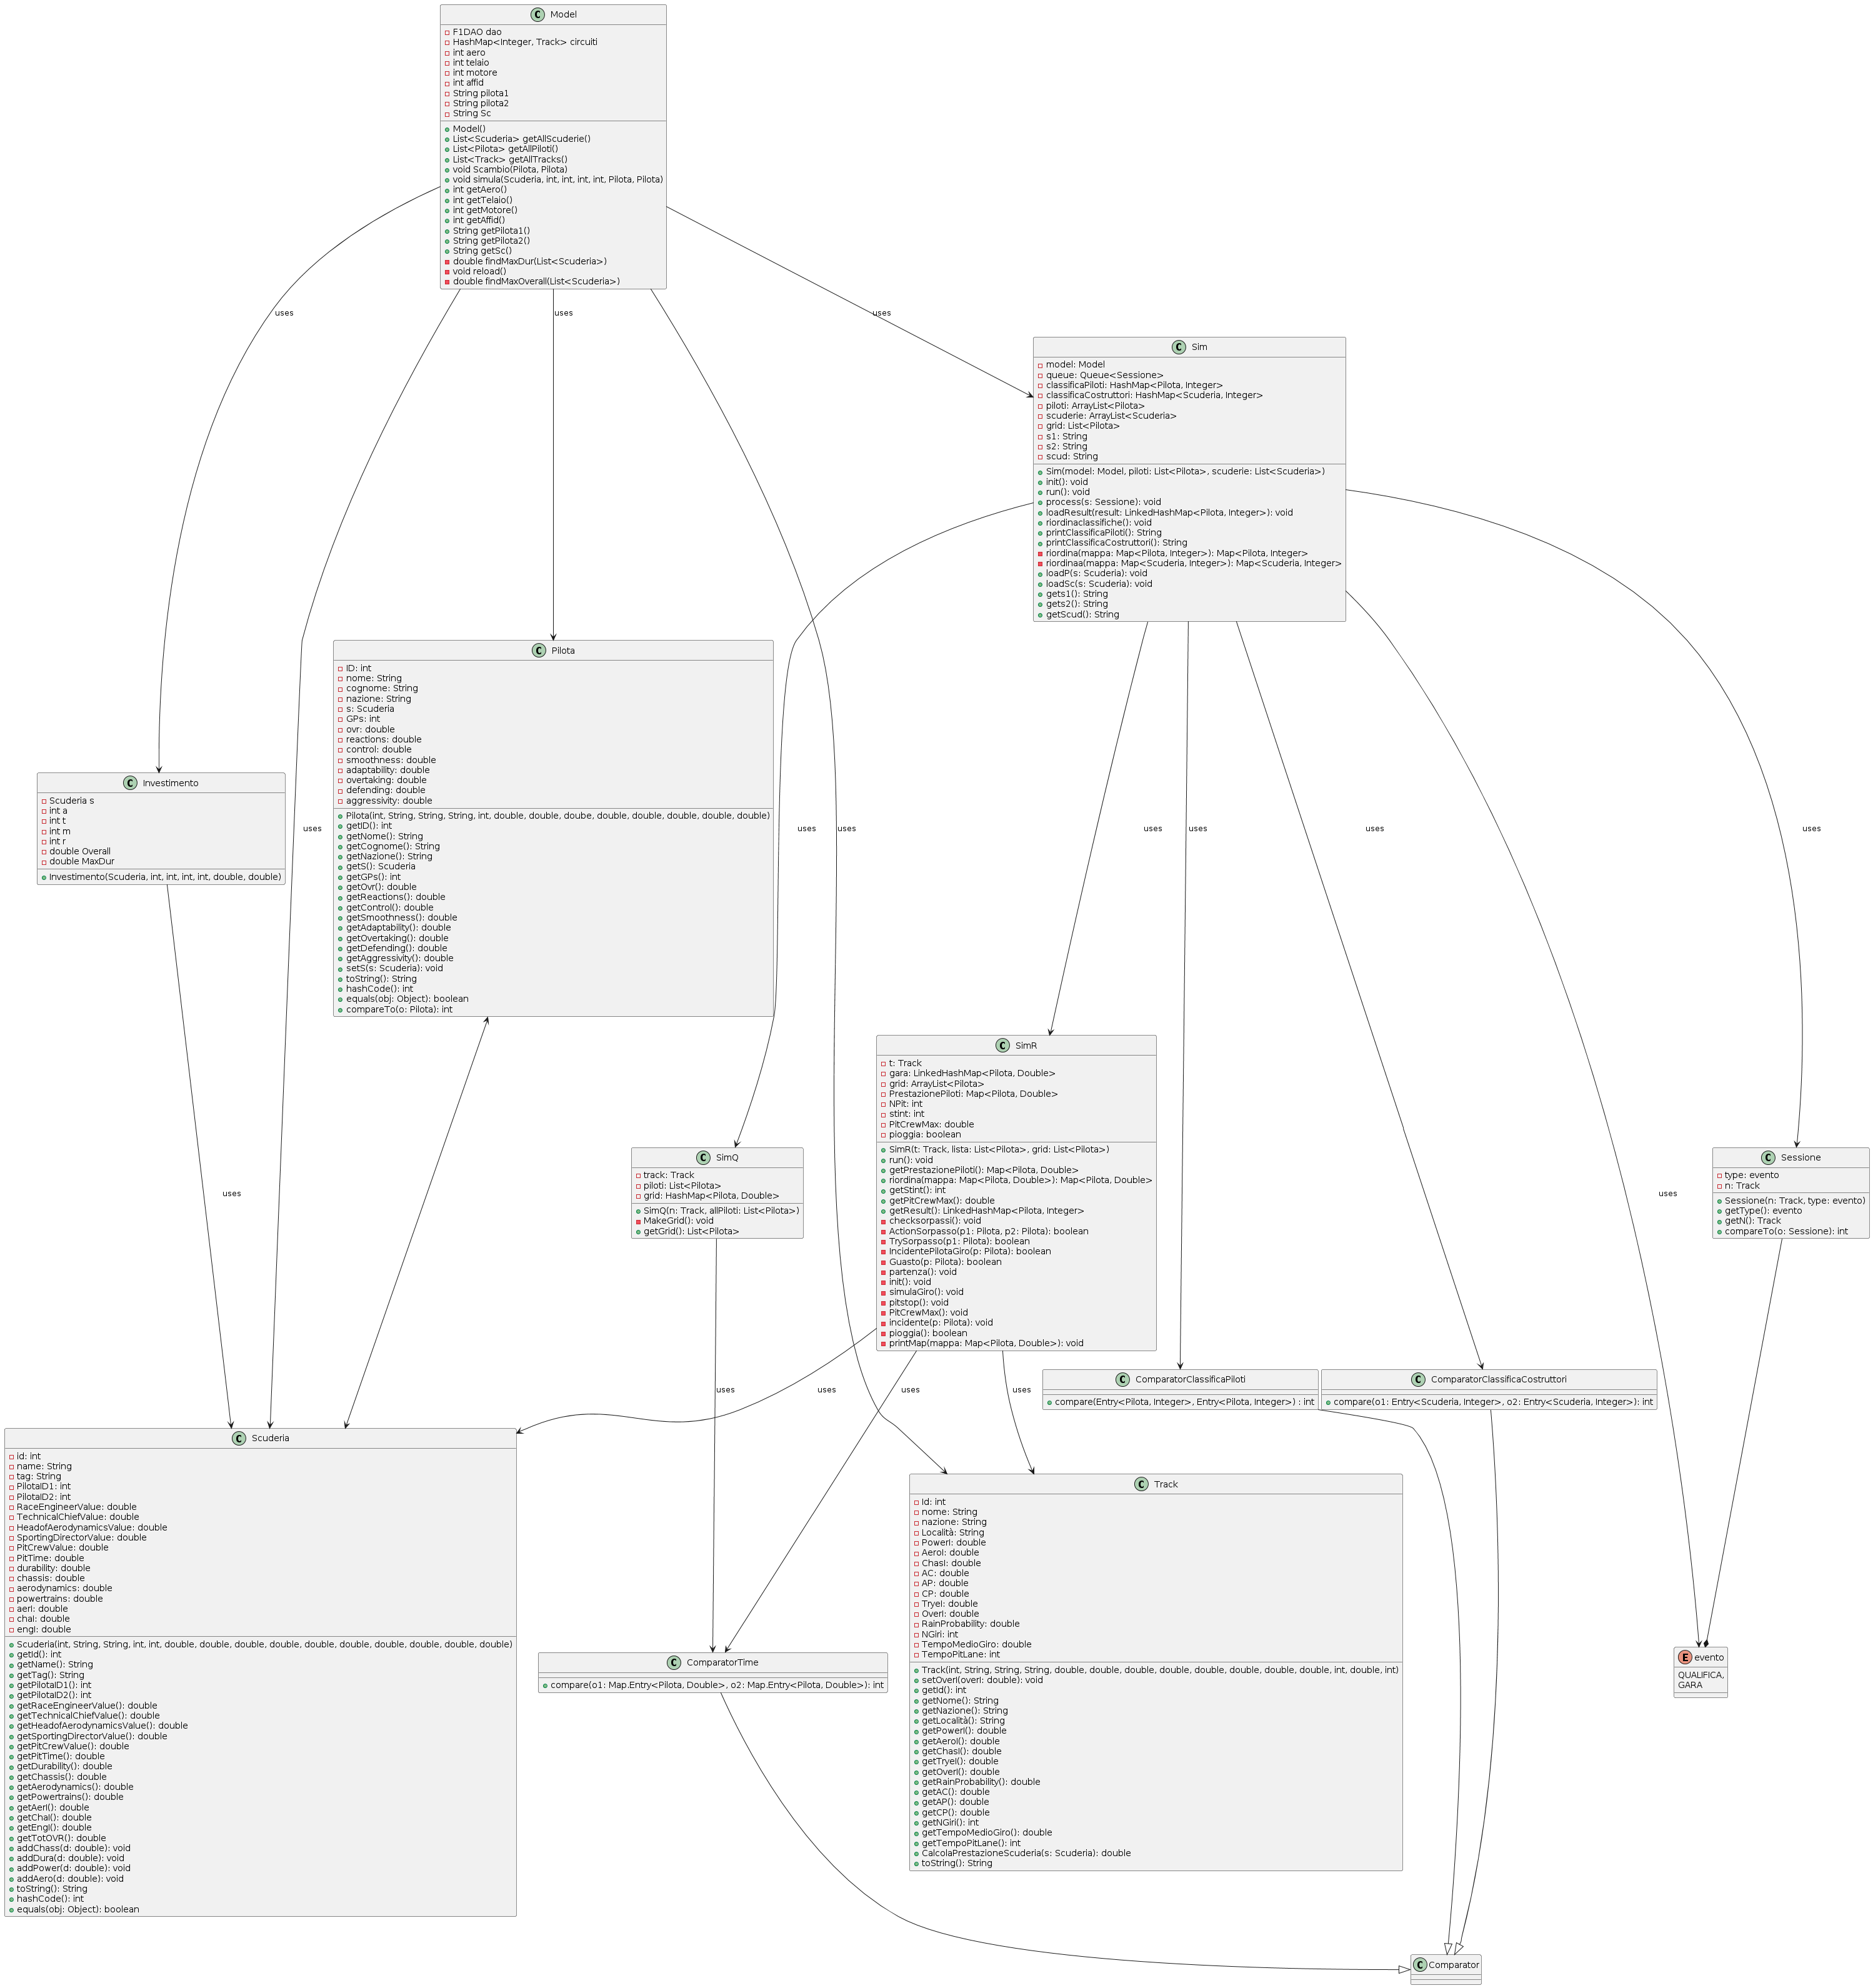
\includegraphics[width=\linewidth, height = 15cm]{Figures/uml3.1.png}
    \caption{Diagramma UML del package SimulazioneF1.model}
    \label{fig:diagramma_model}
\end{figure}
\newpage
\section{Package SimulazioneF1.db}
\vspace{2cm}
\begin{figure}[h!]
    \centering
    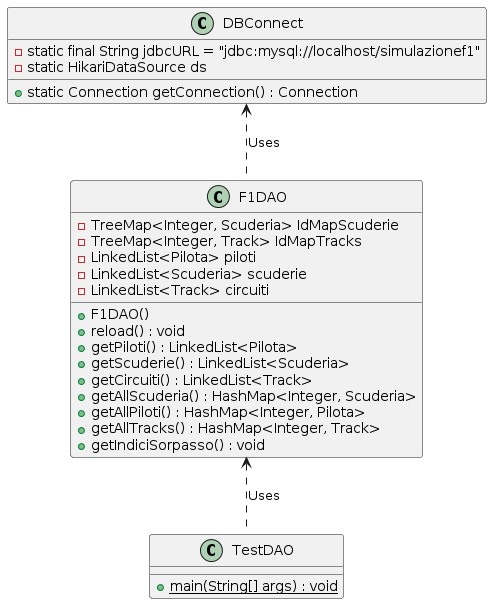
\includegraphics[width=0.8\linewidth]{Figures/uml2.png}
    \caption{Diagramma UML del package SimulazioneF1.db}
    \label{fig:diagramma_db}
\end{figure}


